%!TEX root = tcc.tex

\chapter{Solução} \label{ch:solucao}

\section{Figuras} \label{sec:figuras}

A \cref{fig:logo-unisul} apresenta o logo da UNISUL.

\begin{figure}[H]
\centering
\caption{Logo da Unisul}
\label{fig:logo-unisul}
\includegraphics[width=90mm]{logo_unisul}
\caption*{Fonte: http://unisul.br/}
\end{figure}

\lipsum[1]

\section{Tabelas} \label{sec:tabelas}

A \cref{tab:taxa-desemprego} apresenta a taxa de desemprego aberto.

\begin{table}[H]
\centering
\caption{Taxa de desemprego aberto, por região metropolitana, do primeiro semestre de 1992.}
\label{tab:taxa-desemprego}
\begin{tabular}{|c|c|c|c|c|}
\hline
\multirow{2}{*}{Ano e mês} & \multicolumn{4}{|c|}{Região metropolitana}          \\ \cline{2-5}
                           & Recife & Salvador & Belo Horizonte & Rio de Janeiro \\ \hline
Janeiro                    & 6.10   & 5.43     & 4.77           & 4.24           \\ \hline
Fevereiro                  & 6.44   & 5.18     & 5.00           & 3.81           \\ \hline
Março                      & 6.33   & 5.76     & 5.06           & 4.24           \\ \hline
Abril                      & 6.67   & 6.06     & 4.47           & 4.13           \\ \hline
Maio                       & 6.21   & 7.26     & 4.61           & 5.54           \\ \hline
Junho                      & 5.30   & 6.43     & 4.31           & 3.63           \\ \hline
\end{tabular}
\caption*{Fonte: FUNDAÇÃO INSTITUTO BRASILEIRO DE GEOGRAFIA E ESTATÍSTICA. \textbf{Normas de apresentação tabular}. 3.ed. Rio de Janeiro, 1993. p. 51}
\end{table}

\lipsum[1]

\section{Gráficos} \label{sec:graficos}

\begin{figure}[H]
  \centering
  \caption{Representação gráfica da \cref{tab:taxa-desemprego}}
  \label{fig:taxa-desemprego}
  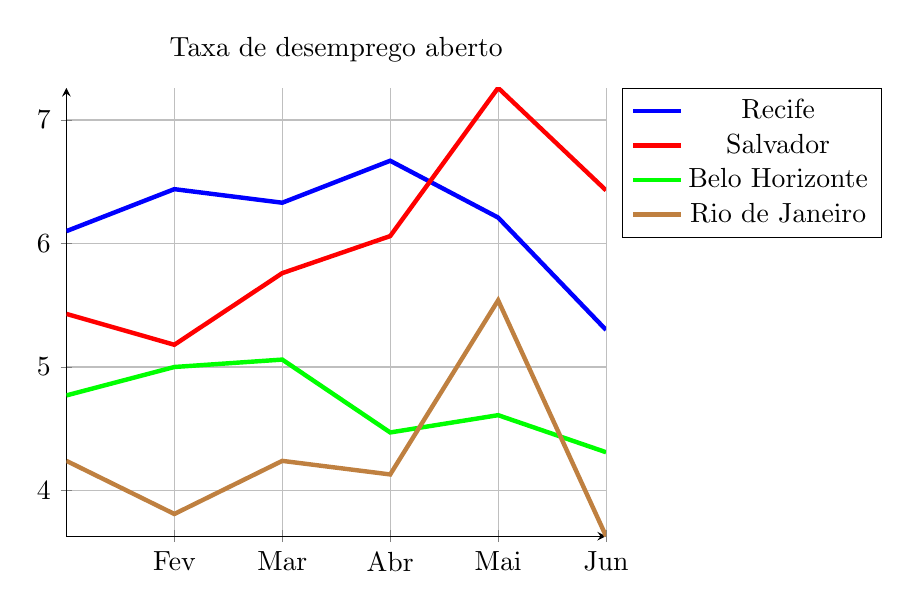
\begin{tikzpicture}
    \begin{axis}[
        grid=both,
        axis lines=middle,
        legend pos=outer north east,
        symbolic x coords={Jan, Fev, Mar, Abr, Mai, Jun},
        title={Taxa de desemprego aberto}
      ]
      \addplot[blue, ultra thick]
         coordinates{(Jan, 6.10)(Fev, 6.44)(Mar, 6.33)(Abr, 6.67)(Mai, 6.21)(Jun, 5.30)};
      \addlegendentry{Recife}
      \addplot[red, ultra thick]
         coordinates{(Jan, 5.43)(Fev, 5.18)(Mar, 5.76)(Abr, 6.06)(Mai, 7.26)(Jun, 6.43)};
      \addlegendentry{Salvador}
      \addplot[green, ultra thick]
         coordinates{(Jan, 4.77)(Fev, 5.00)(Mar, 5.06)(Abr, 4.47)(Mai, 4.61)(Jun, 4.31)};
      \addlegendentry{Belo Horizonte}
      \addplot[brown, ultra thick]
         coordinates{(Jan, 4.24)(Fev, 3.81)(Mar, 4.24)(Abr, 4.13)(Mai, 5.54)(Jun, 3.63)};
      \addlegendentry{Rio de Janeiro}
    \end{axis}
  \end{tikzpicture}
  \caption*{Fonte: Autor do Trabalho}
\end{figure}

\lipsum[1]

\section{Códigos} \label{sec:codigos}

\begin{figure}[H]
  \caption{Exemplo de JSON de retweet com números utilizados}
  \label{fig:retweet-json-numbers}
  \lstinputlisting[language=json, firstline=2, lastline=14]{code/retweet-sample-numbers.json}
  \caption*{Fonte: Autor do Trabalho}
\end{figure}

\lipsum[1]

\section{\emph{Glossaries}} \label{sec:glossaries}

Utilizando abreviatura pela primeira vez \gls{unisul}. Utilizando abreviatura pela segunda vez \gls{unisul}.

Utilizando sigla pela primeira vez \gls{sc}. Utilizando sigla pela segunda vez \gls{sc}.

Utilizando glossário pela primeira vez \gls{dissertacao}. Utilizando glossário pela segunda vez \gls{dissertacao}.

Utilizando simbolo pela primeira vez \glssymbol{sum}. Utilizando simbolo pela segunda vez \glssymbol{sum} \cite{latex-guide}. Abaixo equação com \gls{sum}:

$$
  \glssymbol{sum}_{i=0}(x+i)
$$

\section{Demais Referências} \label{sec:demais-ref}

A \cref{sec:figuras} apresentou como as figuras são utilizadas. A \cref{subsec:obj-general} apresentou o objetivo geral conforme \citeonline{latex-guide}.
